\documentclass[11pt]{article}
\usepackage[utf8]{inputenc}
\usepackage[T1]{fontenc}
\usepackage{amsmath,amssymb}
\usepackage{graphicx}
\usepackage{booktabs}
\usepackage{geometry}
\geometry{margin=1in}
\usepackage[hidelinks]{hyperref}

\title{Assumed-not-Earned: Verification Efficiency under Bounded Risk\\
\large A cross-domain study of when verification should stop}
\author{Seung-hyun Lee\\ \texttt{hyeon3125@gmail.com}}
\date{June 2026}

\newcommand{\elo}{\mathrm{Elo}}

\begin{document}
\maketitle

\begin{abstract}
We study a single question across number theory, cosmology, control, statistics,
and large-language-model (LLM) evaluation: \emph{when should verification stop,
given a cost of checking and a risk of being wrong?} We formalize a
non-refutation \emph{overhead boundary}---stop accumulating evidence once the
posterior probability of a surviving counterexample falls below a threshold
$\epsilon$---and ask not whether stopping is cheaper (it is) but whether it is
\emph{correct}. Under a correctly specified prior the rule has a provable risk
bound, $\mathrm{miss\_rate}\le\epsilon(1-\pi_0)$, verified empirically at
$\sim$94\% compute saved; under prior misspecification the same rule fails
silently, and the historical record of famously disproven conjectures
(P\'olya, Mertens, $\pi(x)<\mathrm{li}(x)$) shows the failure is the norm, not a
contrived case. The mirror question---when does \emph{adding} structure pay---gives
the same answer: a localized (``windowed'') model loses on cosmological data
(structure assumed) but wins on the Nile regime-shift series (structure earned),
and the two cases are one detection curve in the structure's signal-to-noise
ratio (SNR). One law organizes every result: \textbf{a verification shortcut is
worth exactly the degree its assumptions match reality; its failure mode is always
assumed-not-earned.} We close with a live application: using the exact LMArena
Elo$\to$win-rate map and pre-registered perceptibility floors, recent frontier LLM
improvement is inside the overhead region \emph{on the everyday-text projection}
(top-10 within 14~Elo, $\sim$51\% blind preference) but not on others (coding
spread $\sim$256~Elo); and because capability is a vector whose multimodal,
agentic, and vendor-specific axes are not benchmarked across vendors---and whose
``everyday'' axis is itself an unmeasured proxy that conflates capability
saturation with a low-information prompt mix---the global claim ``scaling has
saturated'' is itself assumed-not-earned. The contribution is
the cross-domain synthesis and a pre-registered, fabrication-averse protocol that
reports its own negatives---not new theory in any single field.
\end{abstract}

\section{Introduction}
This paper is not about physics, number theory, or control engineering; those are
\emph{application instances}. The subject is \emph{computational verification} and
\emph{statistical decision theory}: the unit of study is a verification system, and
the quantity of interest is its efficiency under a bounded risk of misjudgment.
Each domain is the same question in different clothes---cosmology asks ``how much
do we verify a model,'' the Riemann Hypothesis (RH) asks ``when do we stop
searching for a counterexample,'' control asks ``when does another sample stop
adding information.''

We make three claims. (i) A non-refutation stopping rule (the \emph{overhead
boundary}) has a provable risk bound when its prior is correct, and a silent,
unbounded failure when it is not (\S\ref{sec:bound}--\ref{sec:history}). (ii) The
mirror operation---positing extra structure---obeys the identical law: it pays iff
the structure is genuinely present, and ``present'' is a position on a
signal-to-noise curve (\S\ref{sec:earned}). (iii) Applied to LLM progress, the law
makes the diminishing-returns question precise and shows it is well-posed only on
the one capability axis we actually measure (\S\ref{sec:llm}). The contribution is
the synthesis and the discipline (pre-registration, honest negatives, no
fabricated numbers), not a new theorem; \S\ref{sec:related} positions it against
mature prior work.

\paragraph{Protocol.} All operational definitions, baselines, tolerances, and an
assumption-counting rubric were fixed before any result (one amendment disclosed);
every number is parsed mechanically from a real run. A four-domain efficiency
scorecard, $E=\mathrm{phenomena}/(\mathrm{params}+\mathrm{assumptions}+
\mathrm{compute})$ with per-domain ratio $E_{\mathrm{mtp}}/E_{\mathrm{base}}$,
is the quantitative backbone. Two of its domains (the RH scanner, the control
loop) are \emph{construction-flagged demonstrations}, not contributions: their
``wins'' are near-tautological once one accepts stopping. The load-bearing
evidence is the un-flagged, ground-truth work below. Code, pre-registration, and
data: \url{https://github.com/hyeon3125-dev/MTP-MetaEval}.

\section{The overhead boundary and its bounded risk}\label{sec:bound}
Consider a population of conjectures, each either TRUE (no counterexample in the
horizon $[0,M)$) or FALSE (a counterexample at $x\sim\mathrm{Geometric}(r)$).
Checking candidate $t$ reveals whether it refutes, at unit cost plus a Landauer
entropy increment \citep{landauer1961}. The baseline scans exhaustively to $M$.
The overhead rule: having survived $[0,t)$, the posterior that a counterexample
remains is
\begin{equation}
q(t)=\frac{\pi_0\,S(t)}{(1-\pi_0)+\pi_0\,S(t)},\qquad S(t)=\Pr(x\ge t),
\end{equation}
and we stop at the smallest $t$ with $q(t)\le\epsilon$, where $\epsilon$ is set by
the marginal entropy-cost/stake ratio. This is a Bayesian optimal-stopping rule
\citep{wald1945,chow1971}.

\paragraph{Risk bound.} A FALSE conjecture is \emph{missed} only if its
counterexample lies beyond the floor, so
$\mathrm{miss\_rate}=\pi_0\,S(t_{\mathrm{floor}})\le\epsilon(1-\pi_0)$. The
experiment confirms this to the digit (Table~\ref{tab:bound}): at $\epsilon=0.01$
the empirical miss rate is $0.0052$ versus the bound $0.0050$, while saving
$94.5\%$ of the checks. ``Keep searching, stop at a principled floor'' is therefore
\emph{not} nihilism: the misjudgment probability is a knob set in advance.

\begin{table}[h]\centering
\begin{tabular}{rrrrr}
\toprule
$\epsilon$ & $t_{\mathrm{floor}}$ & miss rate & bound $\epsilon(1-\pi_0)$ & compute saved\\
\midrule
0.05  & 146 & 0.0269 & 0.0250 & 96.2\%\\
0.01  & 228 & 0.0052 & 0.0050 & 94.5\%\\
0.005 & 263 & 0.0027 & 0.0025 & 93.8\%\\
0.001 & 342 & 0.0008 & 0.0005 & 92.2\%\\
\bottomrule
\end{tabular}
\caption{The floor's risk is bounded by $\epsilon(1-\pi_0)$ under a correct prior.}
\label{tab:bound}
\end{table}

\section{Failure under misspecification}\label{sec:fail}
Now let the true counterexample tail be heavier than the prior assumes. At a tail
only $2\times$ heavier the miss rate exceeds the bound by $\sim$10$\times$; at
$4\times$ it reaches $0.16$ ($\sim$31$\times$ the bound) while still ``saving''
93\% of compute---the risk knob lies. A \emph{conservative} floor (assume a tail
heavier by factor $s$) restores safety up to heaviness $s$ but gives back compute:
saved drops $94.5\%\!\to\!63\%$ as $s:1\!\to\!8$. Robustness buys range, never
invulnerability; against an unbounded tail no finite-compute floor is safe.

\section{Real-world failure: the historical record}\label{sec:history}
\S\ref{sec:fail} is the historical norm. Of four famously \emph{disproven}
conjectures, an efficient floor would have endorsed all four as ``non-refuted''
(Table~\ref{tab:hist}). Two---Mertens \citep{odlyzko1985} and
$\pi(x)<\mathrm{li}(x)$ \citep{littlewood1914}---have counterexamples beyond any
feasible computation and were settled only by proof. Collatz (verified to
$2^{68}$ \citep{barina2020}) and Goldbach (to $4\times10^{18}$
\citep{oliveira2014}) are correctly endorsed by stopping. The lesson:
non-refutation stopping is safe only given a \emph{proven bound} on
counterexample location. RH has none, so the RH demonstration's ``win'' is the
same unbounded gamble as Mertens.

\begin{table}[h]\centering
\begin{tabular}{lll}
\toprule
conjecture & counterexample & floor outcome\\
\midrule
P\'olya & $n\approx9\times10^8$ \citep{tanaka1980} & misses (far past ``settled'')\\
Euler $n{=}5$ & $144^5$ \citep{lander1966} & misses\\
Mertens & beyond computation ($\le e^{1.59\times10^{40}}$) & misses---proof only\\
$\pi(x)<\mathrm{li}(x)$ & $\approx1.4\times10^{316}$ \citep{demichel2005} & misses---proof only\\
\bottomrule
\end{tabular}
\caption{An efficient floor endorses every famous disproven conjecture.}
\label{tab:hist}
\end{table}

\section{Earned versus assumed structure}\label{sec:earned}
The mirror of stopping is \emph{adding} structure. In cosmology, a windowed
interacting-dark-energy model posits a localized dark-sector coupling. Against DESI
DR1 BAO \citep{desi2024}, RSD growth, and Planck distance priors
\citep{chen2019}, the data drive the coupling to zero; the model never beats
$\Lambda$CDM on AIC/BIC \citep{akaike1974,schwarz1978} and its scorecard ratio is
$\approx0.02$. The assumed structure was not in the data.

The \emph{same} move succeeds where the structure is real. On the Nile
annual-minimum series (1871--1970), with a documented 1899 regime shift, a
changepoint model selects index~28 (year~1899) with $\Delta\mathrm{AIC}=-53$ and
permutation $p<0.001$, and is \emph{not} selected under a shuffled null. Identical
operation, opposite verdict, decided only by whether the structure exists.

\paragraph{One curve, not two anecdotes.} Cosmology (lost) and Nile (won) are the
ends of one quantity: the structure's signal-to-noise ratio (SNR). Sweeping SNR
with noise calibrated to Nile's within-segment scatter
(Figure~\ref{fig:snr}) gives a null-calibrated detection-power curve crossing 95\%
at $\mathrm{SNR}\approx0.9$. Nile sits at $\mathrm{SNR}\approx2.0$ (power $\approx1$);
the cosmological signal was sub-percent versus the data errors, $\mathrm{SNR}\ll1$,
below threshold. A self-referential corollary: the \emph{detector} must itself be
earned---naive AIC$<$0 selects the localized model $\sim$48\% of the time from pure
noise (the location search overfits, unpenalized), corrected only by null
calibration \citep{rissanen1978}.

\begin{figure}[h]\centering
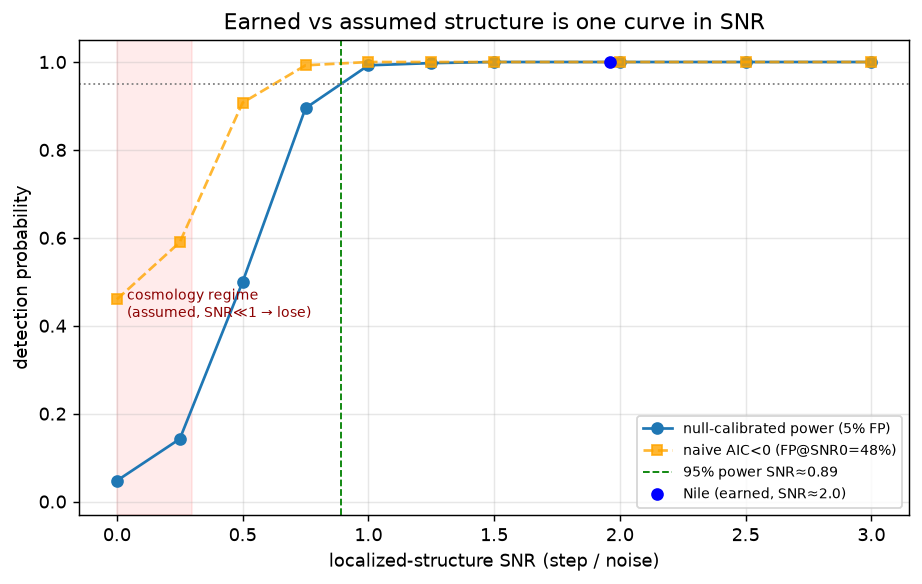
\includegraphics[width=0.78\textwidth]{figs/earned_threshold.png}
\caption{Earned vs.\ assumed structure is one curve in SNR. Null-calibrated power
(blue) reaches 95\% near $\mathrm{SNR}=0.9$; Nile (earned) sits high, the
cosmology regime (assumed, $\mathrm{SNR}\ll1$, red) below. Naive AIC (orange)
shows a $\sim$48\% false-positive rate at $\mathrm{SNR}=0$.}
\label{fig:snr}
\end{figure}

\section{The general law}
\begin{center}\itshape
A verification shortcut is worth exactly the degree its assumptions match reality;
its failure mode is always assumed-not-earned.
\end{center}
Whether the shortcut is a stopping floor (\S\ref{sec:bound}--\ref{sec:history}) or
an added structure (\S\ref{sec:earned}), the value tracks the assumption--reality
match and the failure is the same: a structure or bound believed but not present.
The law even reaches the detector (the false-positive corollary above).

\section{Application: has LLM capability entered the overhead region?}\label{sec:llm}
The overhead boundary with model generations as the accumulation axis and
user-perceptible difference as the floor. The one exact ingredient is LMArena's
blind win-rate map \citep{chiang2024},
$P(\mathrm{win})=1/(1+10^{-\Delta\elo/400})$ ($100~\elo\to0.640$); the floor is
pre-registered (``barely perceptible'' at $P=0.55$, i.e.\ $\Delta\elo\ge35$).

\paragraph{Aggregate text: inside the overhead region.} The real Arena
overall/text top-10 (June 2026) spans $14~\elo$ (1510 down to 1496), so the
largest adjacent gap is $\sim$7~\elo, a $\sim$51\% blind preference---below the
$35~\elo$ floor. The marginal gain per generation has crossed the floor:
GPT-3.5$\to$GPT-4 was $\sim$100~\elo (earned); 2025--26 adjacent gaps are
4--14~\elo. On the median everyday prompt, recent frontier improvement buys
capability with $\sim$0 perceptible marginal difference \citep{kaplan2020,hoffmann2022}.

\paragraph{But ``hard'' is not a metric; capability is a vector.} The overhead
verdict is a \emph{projection} onto an axis, and the axes are measured very
unequally. On the coding projection the same frontier spans $\sim$256~\elo
(top tier $1310$--$1566$)---$18\times$ the overall spread---so the models are
clearly distinguishable there (earned). Arena's category leaderboards re-rank
models (an overall \#1 can be \#5 in coding), and the overall leader tops no single
automated benchmark; benchmarks are fragmented across axes (HLE, ARC-AGI-2, AIME,
FrontierMath, SWE-bench, $\tau^2$-Bench) with \emph{no} vendor-neutral basis, least
of all for multimodal. Of seven capability axes, the overhead verdict is
\emph{measurable} on three (all text) and \emph{undetermined or unmeasurable} on
four (agentic/tool-use, long-context fidelity, multimodal, vendor-specific
architecture). Hence ``has scaling entered overhead?'' is ill-posed without naming
the projection; it is confirmed on the everyday-text axis, re-ranked (plausibly
still earned) on specialist text axes, and unanswerable elsewhere for lack of
measurement. \textbf{Asserting global saturation from aggregate Elo is itself
assumed-not-earned}---it assumes one easy-text projection captures the whole
vector. Falsifiable predictions: hard-category gaps stay above the floor while
overall stays below; any $>35~\elo$ overall gap refutes the claim for that step;
re-weighting toward hard prompts widens adjacent gaps back above the floor.

\paragraph{And ``everyday'' is also unmeasured: the confound.} The one axis we
called ``measurable'' is mis-named too. ``Everyday'' is properly an
information-theoretic quantity---the \emph{shared context} between sender and
receiver, measurable by deictic density (which falls monotonically casual$\to$formal
in our samples), lexical diversity, and most faithfully by language-model
perplexity (so the measuring instrument is the same kind of object being judged).
High-shared-context prompts have a \emph{narrow} correct-answer space---low
capability-SNR by construction---so competent models tie there regardless of
saturation. The aggregate verdict therefore conflates (a) capability saturation
with (b) a prompt mix dominated by low-information tasks, and Arena does not
stratify preference by information content, so it cannot separate them: for the
saturation question the benchmark is, in this respect, an uncontrolled mixture. The
earned claim requires stratified evaluation---do model win-rate gaps shrink across
generations \emph{within} high-information strata?---and until that exists the
defensible statement is only ``adjacent models tie on the aggregate mixture,'' which
is not ``capability has saturated.''

\section{Related work}\label{sec:related}
The overhead boundary is a Bayesian optimal-stopping rule \citep{wald1945,chow1971};
\S\ref{sec:bound}'s bound is a standard risk identity. The efficiency metric is a
transparent cousin of information criteria and minimum description length
\citep{akaike1974,schwarz1978,rissanen1978}. The physical motivation for stopping
is Landauer's principle \citep{landauer1961}. The selective-inference hazard in
\S\ref{sec:earned} is the classic multiple-comparisons problem addressed by
permutation calibration. The LLM section builds on Chatbot Arena \citep{chiang2024}
and the scaling-law literature \citep{kaplan2020,hoffmann2022}. We claim novelty
only in the cross-domain synthesis, the falsification-averse protocol, and the
projection-dependent framing of LLM saturation---not in any single tool.

\section{Limitations}
The cosmology, RH, control, and sequential domains are toy or compressed instances,
chosen for transparency, not coverage. The efficiency metric is sensitive to the
relative scaling of its denominator terms; we report per-domain ratios only and a
compute-excluded sensitivity for cosmology. The LLM analysis uses aggregate blind
preference, which is confounded by style and is not capability; its strength is the
exact Elo map and pre-registered floor, not precise rankings of unreleased models.
Crucially, the multimodal and agentic axes lack the cross-vendor measurement needed
to decide the overhead question there at all, and even on text the aggregate does
not stratify by information content---so the everyday-overhead reading conflates
capability saturation with a low-information prompt mix. These are gaps this paper
names (and gives measurable proxies for) rather than fills; closing them requires
stratified, vendor-neutral evaluation that does not yet exist.

\section{Conclusion}
One pre-registered, fabrication-averse protocol shows that across number theory,
physics, control, statistics, and LLM evaluation, a verification shortcut is worth
exactly the degree its assumptions match reality, and fails---silently and
sometimes unboundedly---when the assumption is believed but not earned. The method
does not tell you whether a hypothesis is true; it tells you how much it costs to
be a given amount of wrong, and when you are allowed to stop paying.

\begin{thebibliography}{99}
\bibitem{akaike1974} H.~Akaike. A new look at the statistical model identification. \emph{IEEE Trans.\ Automatic Control}, 19(6):716--723, 1974.
\bibitem{barina2020} D.~Bar\'ina. Convergence verification of the Collatz problem. \emph{J.\ Supercomputing}, 77:2681--2688, 2020.
\bibitem{chen2019} L.~Chen, Q.-G.~Huang, K.~Wang. Distance priors from Planck final release. \emph{JCAP}, 02:028, 2019. arXiv:1808.05724.
\bibitem{chiang2024} W.-L.~Chiang et al. Chatbot Arena: an open platform for evaluating LLMs by human preference. \emph{ICML}, 2024. arXiv:2403.04132.
\bibitem{chow1971} Y.~S.~Chow, H.~Robbins, D.~Siegmund. \emph{Great Expectations: The Theory of Optimal Stopping}. Houghton Mifflin, 1971.
\bibitem{demichel2005} P.~Demichel. The prime counting function and related subjects, 2005. (First sign change of $\pi(x)-\mathrm{li}(x)$ near $1.397\times10^{316}$; cf.\ Bays \& Hudson 2000.)
\bibitem{desi2024} DESI Collaboration. DESI 2024 VI: cosmological constraints from BAO. \emph{JCAP}, 02:021, 2025. arXiv:2404.03002.
\bibitem{hoffmann2022} J.~Hoffmann et al. Training compute-optimal large language models (Chinchilla). \emph{NeurIPS}, 2022. arXiv:2203.15556.
\bibitem{kaplan2020} J.~Kaplan et al. Scaling laws for neural language models, 2020. arXiv:2001.08361.
\bibitem{lander1966} L.~J.~Lander, T.~R.~Parkin. Counterexample to Euler's conjecture on sums of like powers. \emph{Bull.\ AMS}, 72:1079, 1966.
\bibitem{landauer1961} R.~Landauer. Irreversibility and heat generation in the computing process. \emph{IBM J.\ Res.\ Dev.}, 5(3):183--191, 1961.
\bibitem{littlewood1914} J.~E.~Littlewood. Sur la distribution des nombres premiers. \emph{C.\ R.\ Acad.\ Sci.\ Paris}, 158:1869--1872, 1914.
\bibitem{odlyzko1985} A.~M.~Odlyzko, H.~J.~J.~te Riele. Disproof of the Mertens conjecture. \emph{J.\ Reine Angew.\ Math.}, 357:138--160, 1985.
\bibitem{oliveira2014} T.~Oliveira e Silva, S.~Herzog, S.~Pardi. Empirical verification of the even Goldbach conjecture up to $4\times10^{18}$. \emph{Math.\ Comp.}, 83:2033--2060, 2014.
\bibitem{rissanen1978} J.~Rissanen. Modeling by shortest data description. \emph{Automatica}, 14(5):465--471, 1978.
\bibitem{schwarz1978} G.~Schwarz. Estimating the dimension of a model. \emph{Annals of Statistics}, 6(2):461--464, 1978.
\bibitem{tanaka1980} M.~Tanaka. A numerical investigation on the cumulative sum of the Liouville function. \emph{Tokyo J.\ Math.}, 3:187--189, 1980.
\bibitem{wald1945} A.~Wald. Sequential tests of statistical hypotheses. \emph{Annals of Mathematical Statistics}, 16(2):117--186, 1945.
\end{thebibliography}

\end{document}
